\chapter{Appendix C --- Personal Gear}

The following is a list of suggested personal equipment, written in advance of the 2007 expedition. It's interesting to see how the advice has - and hasn't - changed over the years.

\name{Fiona Hartley}

\section{Personal Stuff for Slovenia Expedition}

This is a short-ish list of personal items to bring to Slovenia.

You can get a 10\% student discount at Blacks and there are often cheap internet deals.

Tents, stoves, cooking equipment, food, plates, mugs, cutlery etc are provided by the club.

\margininbox{Conversations up top}{

Sandeep: Is that mould in the bottom of the mug?

Dave W: You should be asking is that \textit{this year's} mould?}{\logbook}

\subsection{Up the hill}
Can get cold at night, even down to freezing; sometimes rains a lot, so best bring warm clothes. It can also be very hot and sunny so those with wimpy skin should bring a sunhat and lotion. Although the bivi is relatively sheltered from the sun, wind and rain, you will end up sitting around in all weathers. So, it’s best bring clothes that you can put on in layers, including some very warm clothes. Clothes tend to get destroyed by the rocks or the bivi so bring old clothes.

\begin{marginfigure}
\checkoddpage \ifoddpage \forcerectofloat \else \forceversofloat \fi
\centering
 \frame{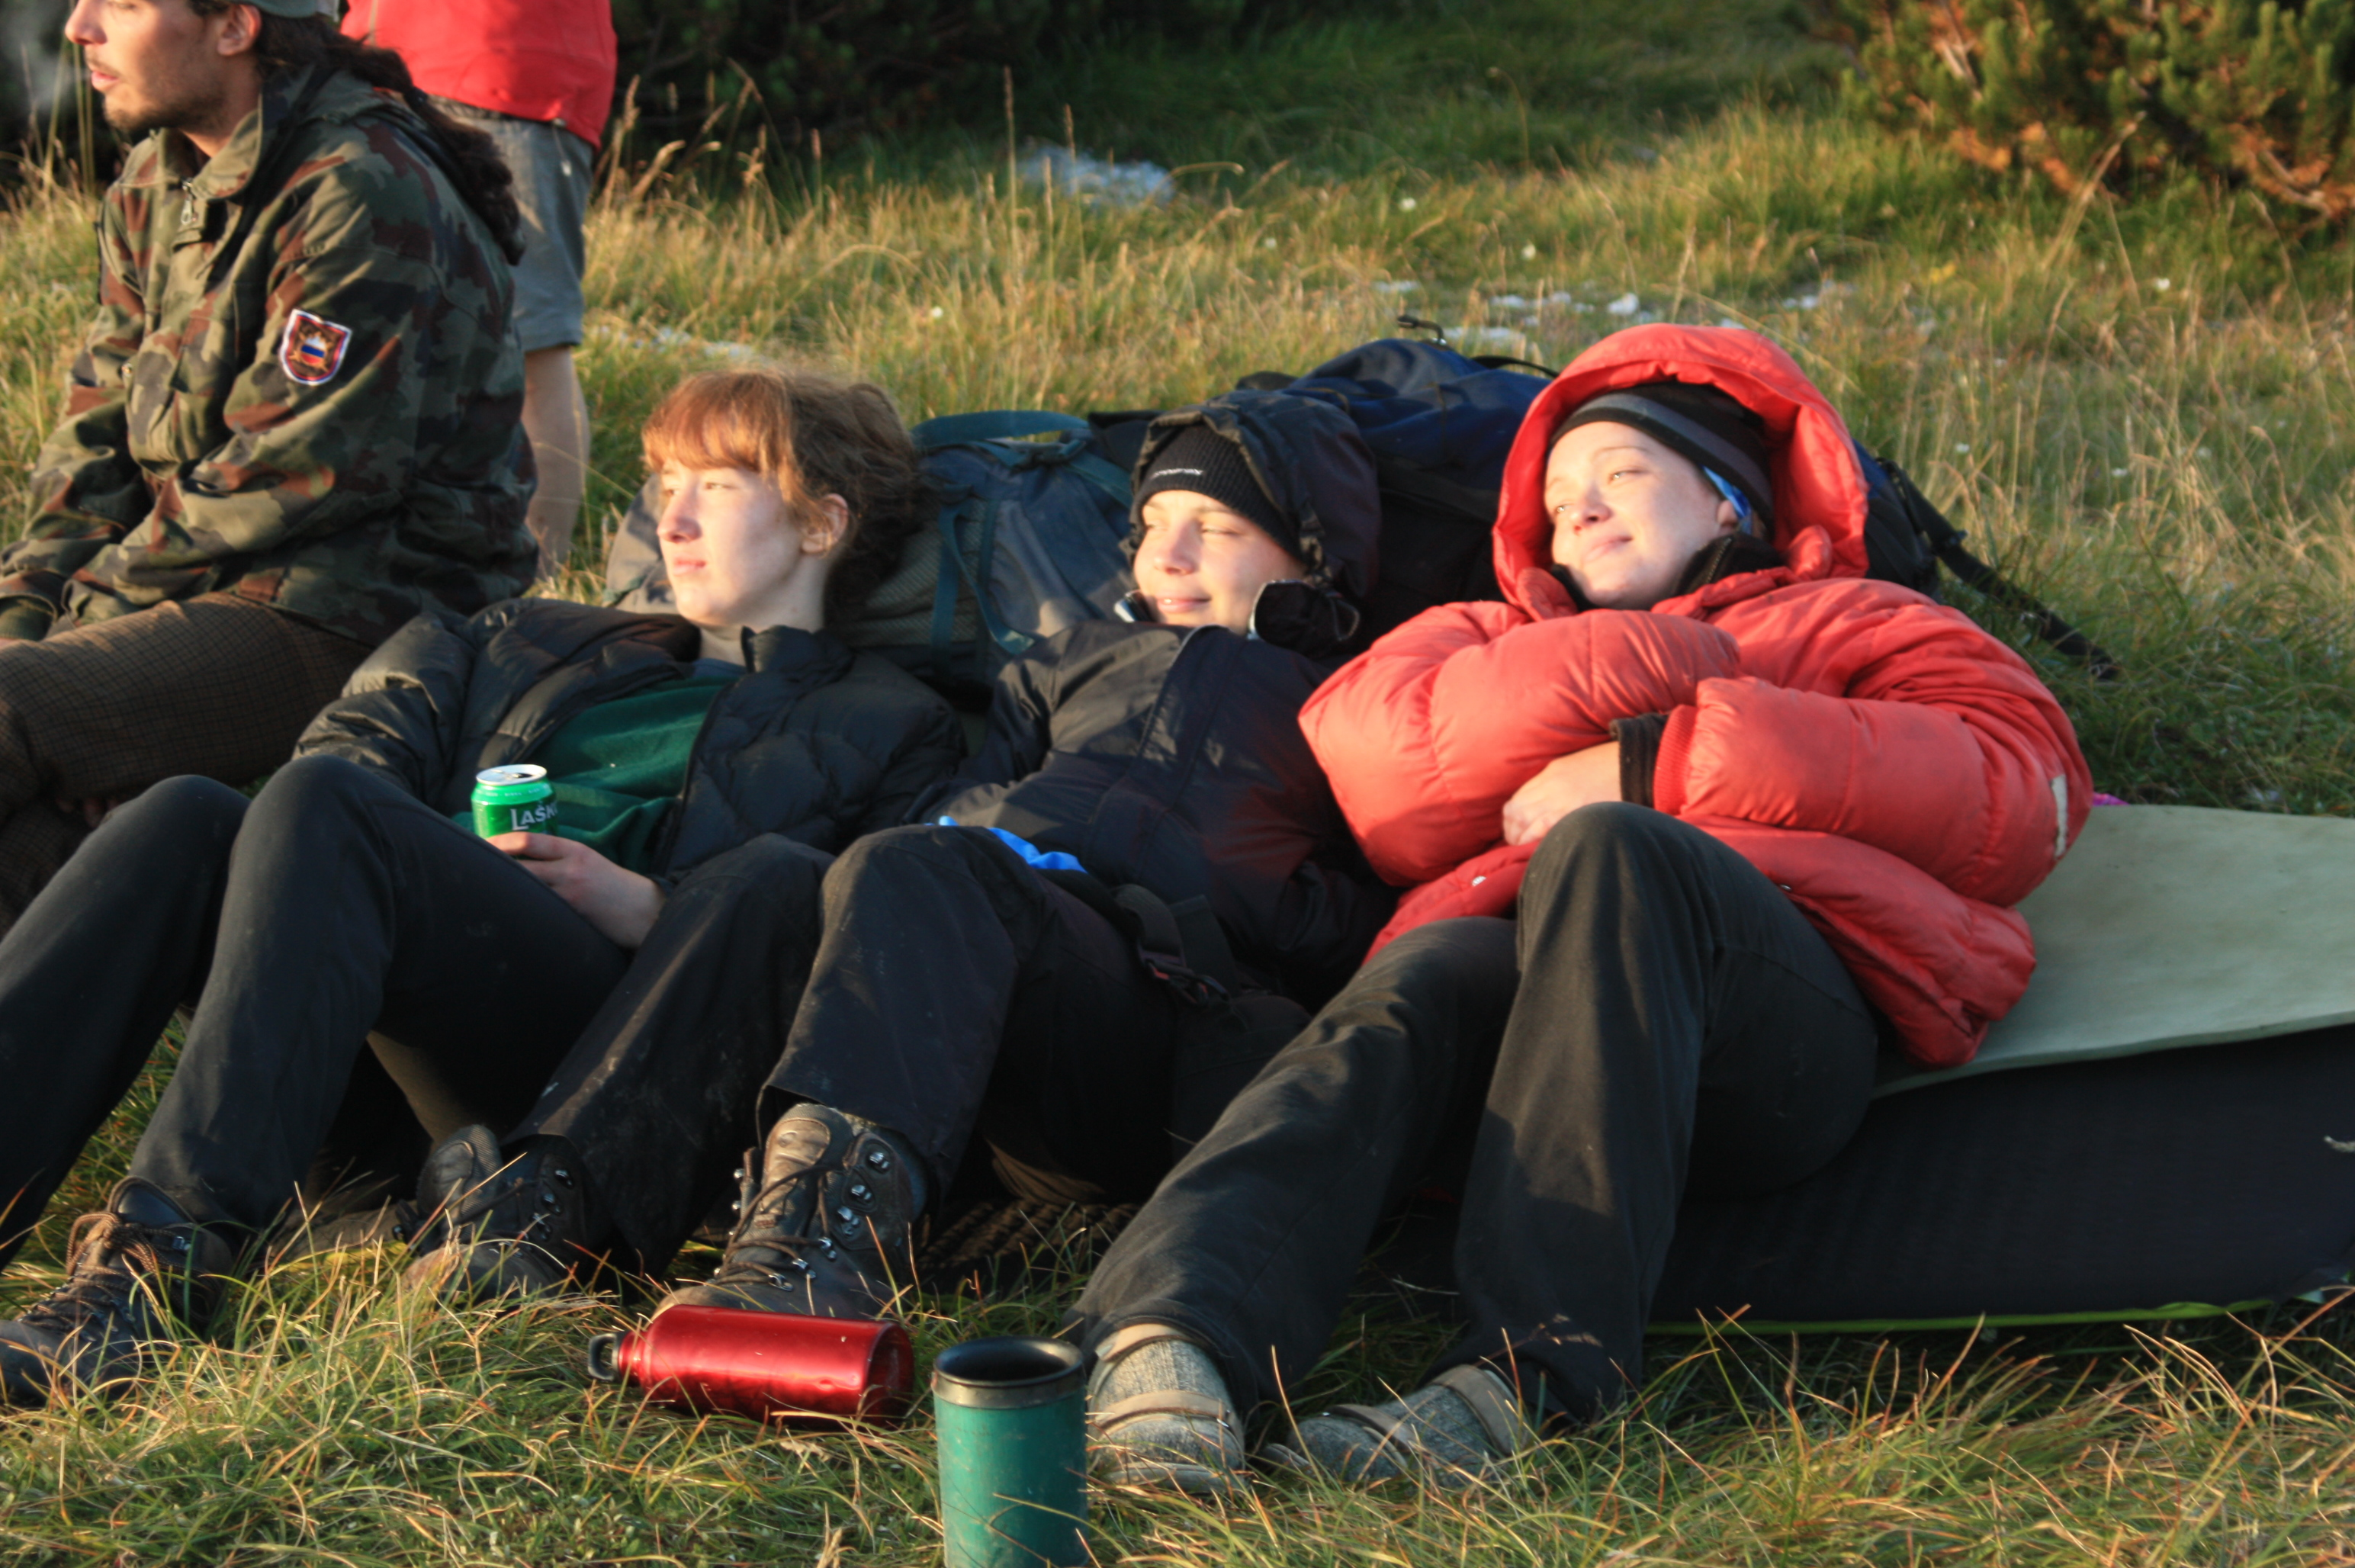
\includegraphics[width=\linewidth]{appendices/personal_equip_2007/2011-08-10-18.57.34-Gergely Ambrus-Canon450D-IMG_1290-Last Evening on Mountain--orig.jpg}} 
 \caption{Kate, Jana and Ari wrapped up in their warm clothes. \pic{Gergely Ambrus}}
 \label{warm gear}
\end{marginfigure}


I’ve got a ranking system for how important things on this list are, it goes as follows:

\textbf{1} – You really need this. If you are in severe financial distress and can’t afford it come and talk to me and we’ll sort something out.

\textbf{2} – Highly recommended, you can sometimes substitute caving kit for this stuff e.g if it’s very cold you can wear a furry instead of a fleece top and fleece trousers. (Not if they're wet you can't!)

\textbf{3} – Old lag stuff (only if you have more money than sense), mainly will make living on top of a mountain more comfortable but it’s not essential.

\newpage

\textbf{Above Ground:}

\begin{marginfigure}
\checkoddpage \ifoddpage \forcerectofloat \else \forceversofloat \fi
\centering
 \frame{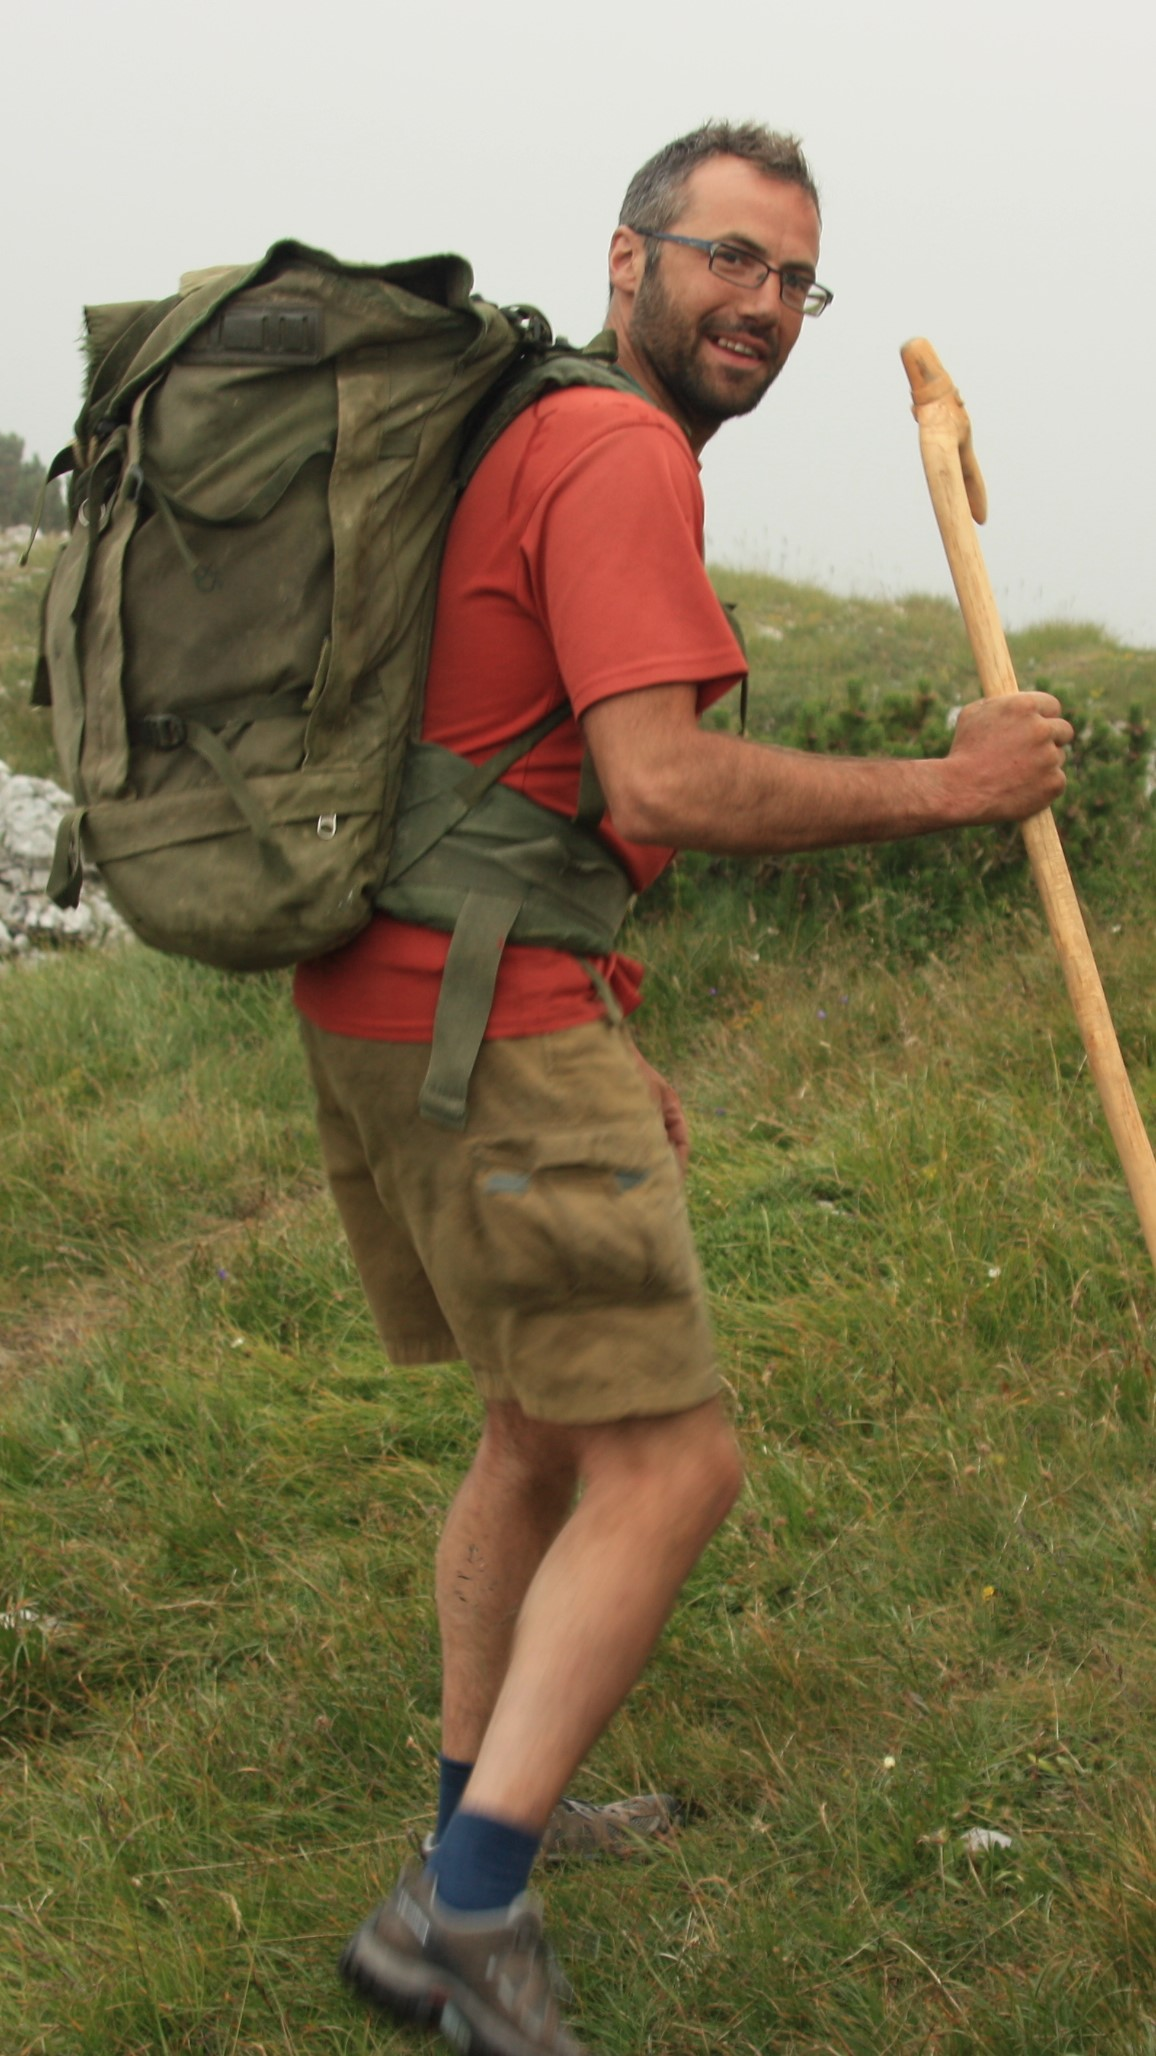
\includegraphics[width=\linewidth]{appendices/personal_equip_2007/2011-08-01-10.55.37-Gergely Ambrus-Canon450D-IMG_0749-Plateau--orig.jpg}} 
 \caption{Tetley in suitable carry clothes. \pic{Gergely Ambrus}}
 \label{tetley carry}
\end{marginfigure}

\begin{itemize}
    \item Good boots (some argue fabric are best. Do not need to be extreme, just something with ankle support.) \textbf{– 1}
    \item Rucksack ~70 ± 10L. It is more important that the bag feels comfortable on your back than it having another 10L of space \textbf{– 1}
    \item Walking Socks \textbf{- 2}
    \item Sandals or other lightweight shoes for bivi or town \textbf{- 2}
    \item Fleece trousers or equivalent \textbf{- 2}
    \item T-shirts/tops/shirts \textbf{- 1} (not too many, 2 or 3 is fine)
    \item Shorts \textbf{- 2}
    \item Underwear (~2-6 sets) \textbf{- Up to you!}
    \item Fleece top or equivalent \textbf{- 1}
    \item Sunhat for during the day and warm hat +/- gloves to wear when it gets cold \textbf{- 1}
    \item Waterproof jacket, does not to be one of those super expensive ones, mine cost £15 from Beatties. Big money saving tip – the wash in waterproof  (produced by a company called Nikwax) improves your waterproof dramatically. \textbf{- 1}
        \item Clewin Logic – If it rains, don’t start walking up or down the hill. If you are already walking, you will as get wet from sweat while wearing a waterproof as you would if it rained on you.
    \item Waterproof trousers \textbf{- 3}
    \item Very, very warm down jacket (highly recommended). Money saving tip, sit closer to the fire! \textbf{- 3}
\end{itemize}


\begin{marginfigure}
\checkoddpage \ifoddpage \forcerectofloat \else \forceversofloat \fi
\centering
 \frame{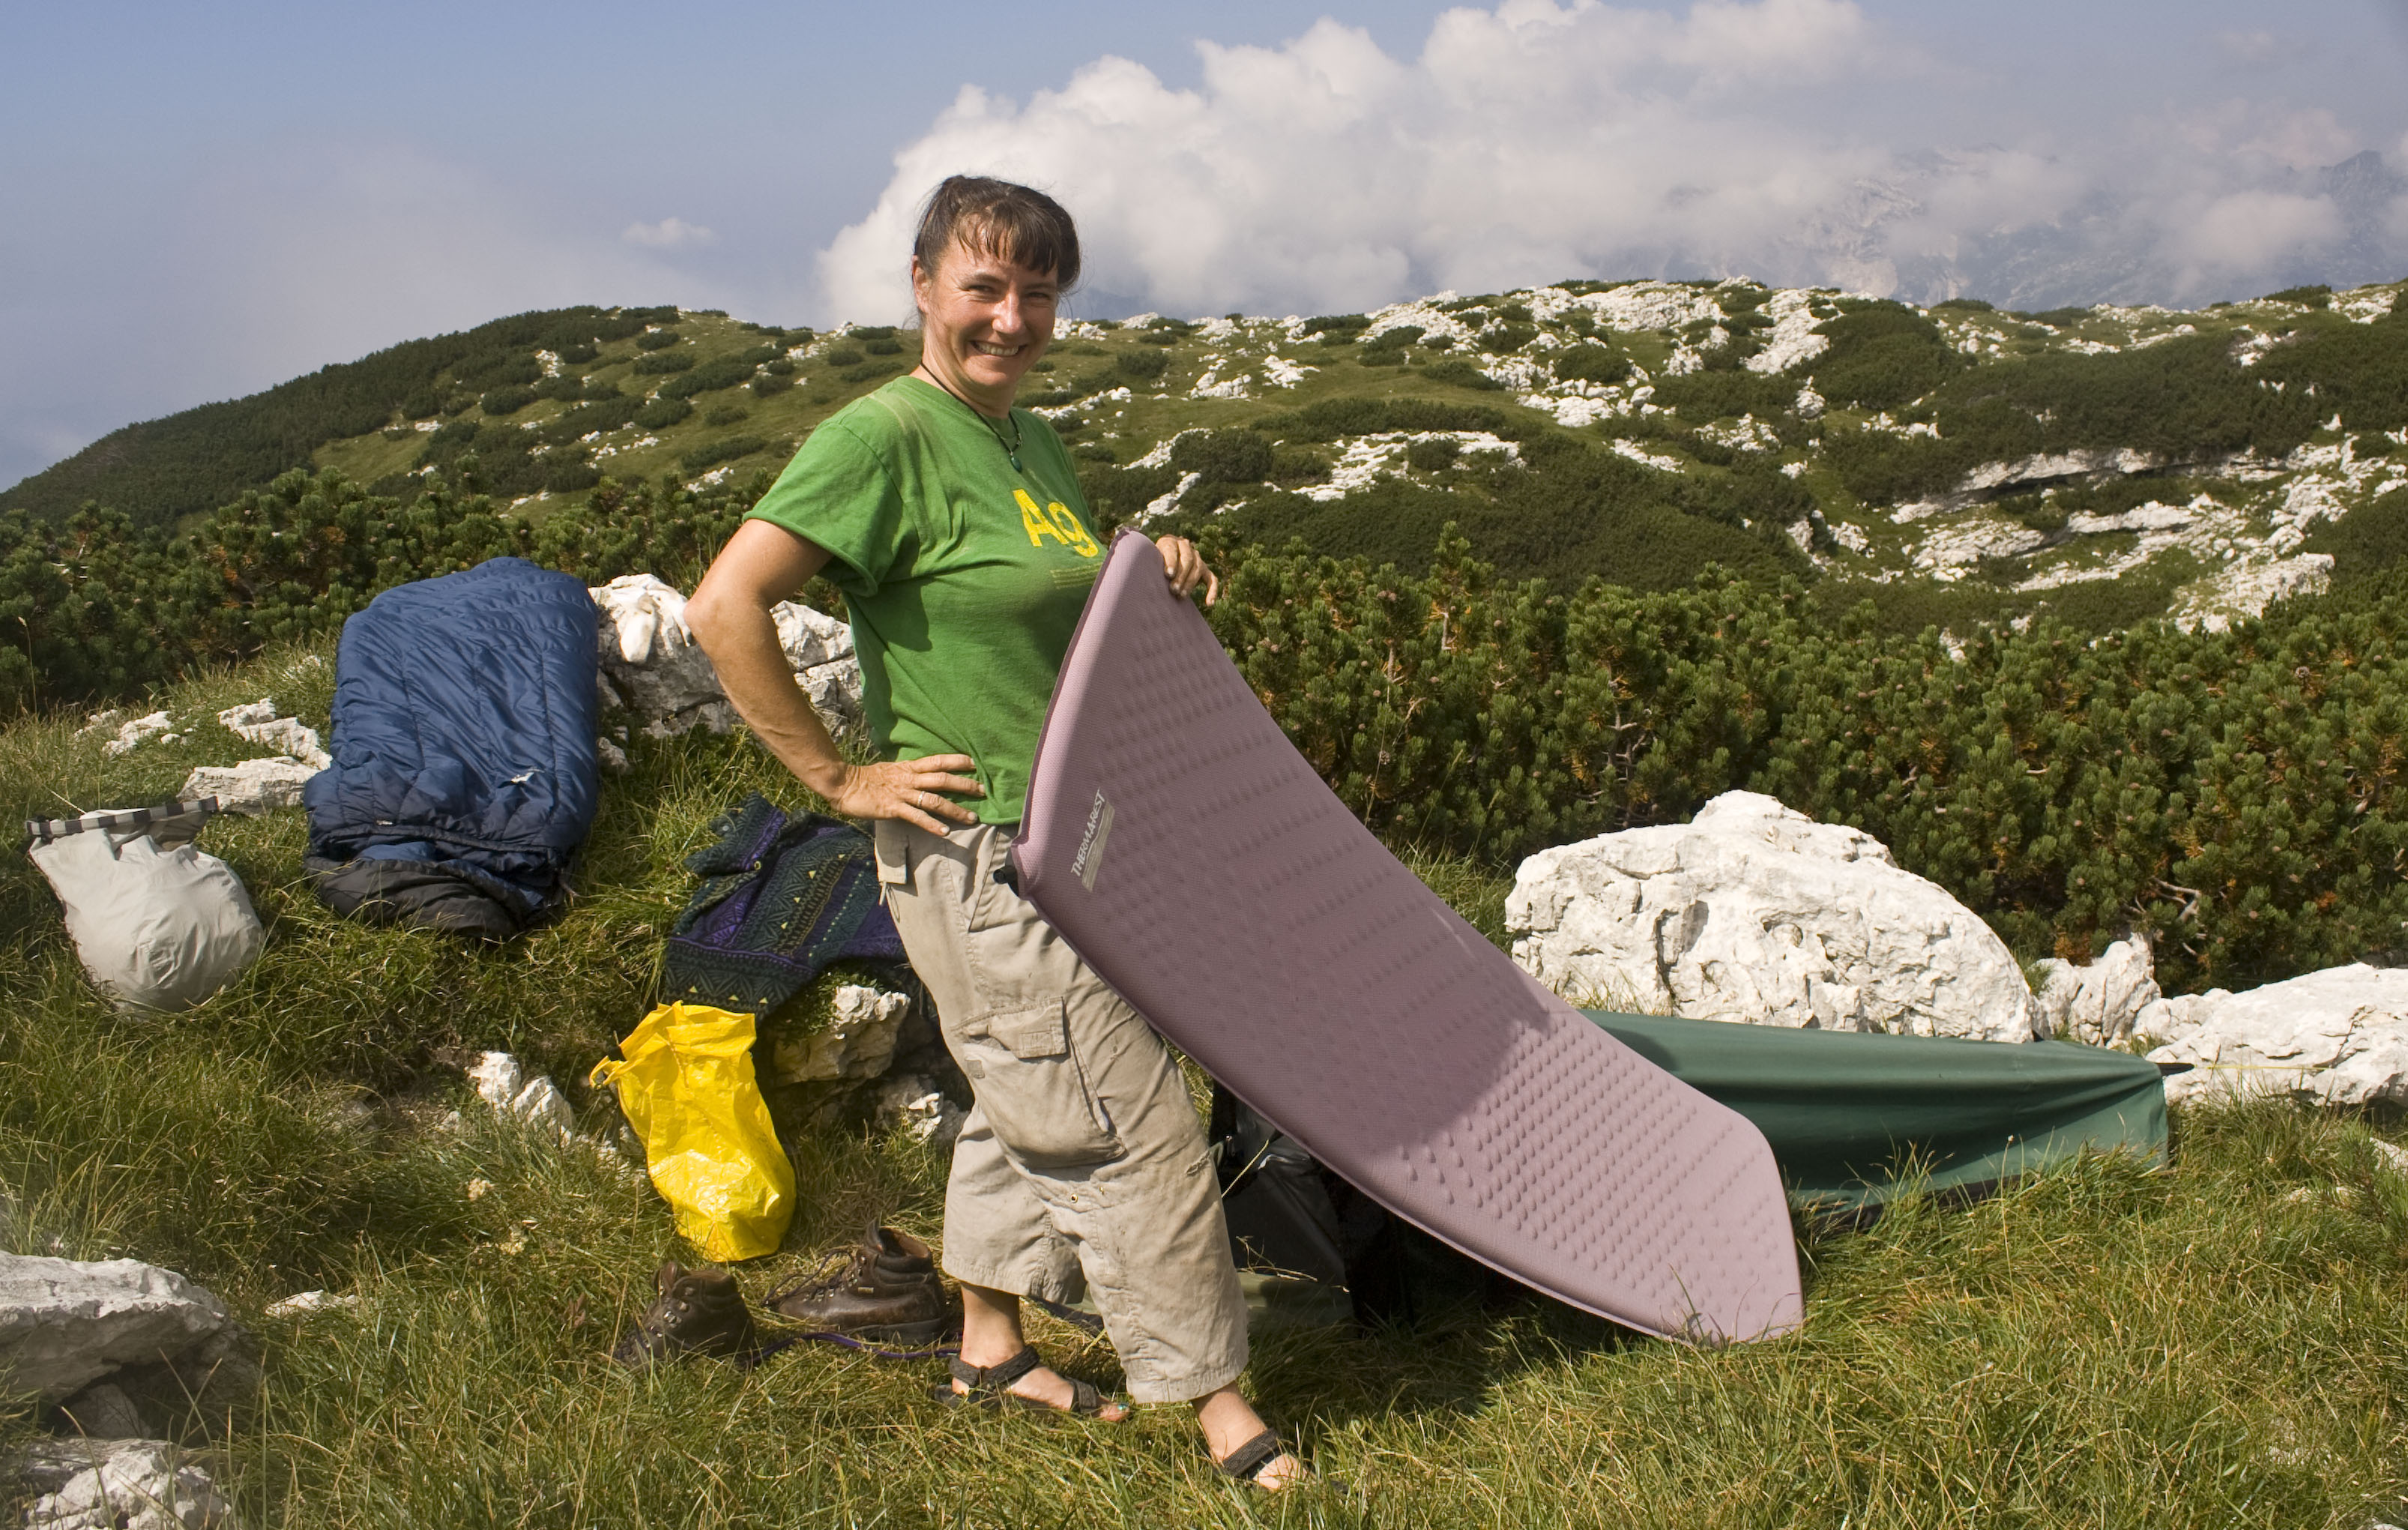
\includegraphics[width=\linewidth]{appendices/personal_equip_2007/2009-Jana Carga - Canon 350d - 048_1--orig.jpg}} 
 \caption{Janet, an old hand, presents expert-level comf for sleeping. \pic{Jana Carga}}
 \label{thermarest}
\end{marginfigure}

\textbf{Miscellaneous:}
\begin{itemize}
    \item Warm Sleeping bag or OK sleeping bag with a fleece liner ~£15 (good money saving tip) \textbf{– 1}
    \item Petzl Tikka headtorch, the plus version is better. Remember spare batteries for these. \textbf{- 1}
    \item Very, very comfy thermarest (\textbf{3}) or equivalent shite foam thingy. (\textbf{1})
    \item Water bottle, you can use a bottled water bottle i.e. volvic. Platapuses are rubbish, you don’t get a rest when you want to drink some water \textbf{- 1}
    \item Diary \& pen \textbf{- 2}
    \item Camera \textbf{- 2}
    \item Sunglasses for posers \textbf{- 3}
    \item Swiss army knife with prussic cord \textbf{- 1}
    \item Suntan lotion \textbf{- 1}
\end{itemize}

\textbf{Wash-kit (top)}
\begin{itemize}
    \item Toothbrush, we smell bad enough but imagine your breath after not brushing for 4 weeks \textbf{- 1}
    \item Toothpaste, you can borrow other peoples if you forgot yours \textbf{- 2}
    \item Spare specs for blind people (or disposable contacts), you’re rarely not going to be focusing at infinity. \textbf{- 1}
    \item Feminine hygiene whatsits \textbf{- ?} (you tell me) 
    \item Footpowder (if you need it, or are told you need it) \textbf{- 2}
    \item Personal 1st aid kit. Although the club has a comprehensive 1st aid kit sometimes plasters or aspirins can be useful. I got my first blister after walking up the hill for the first time, normally a bit of duct tape will do the trick. \textbf{- 2}
    \item Medicines for sick people, if you take something that you might stop working without, you should tell someone else what it is just incase \textbf{– 1!}
\end{itemize}

\subsection{Underground}
\begin{itemize}
    \item Furry
    \item Oversuit
    \item Wellies
    \item Wetsocks/cave socks
    \item Kneepads
    \item Survival bag
    \item Personal SRT-bag with krab
    \item Gloves – Might be nice to get your own ones of these
\end{itemize}


\begin{marginfigure}
\checkoddpage \ifoddpage \forcerectofloat \else \forceversofloat \fi
\centering
 \frame{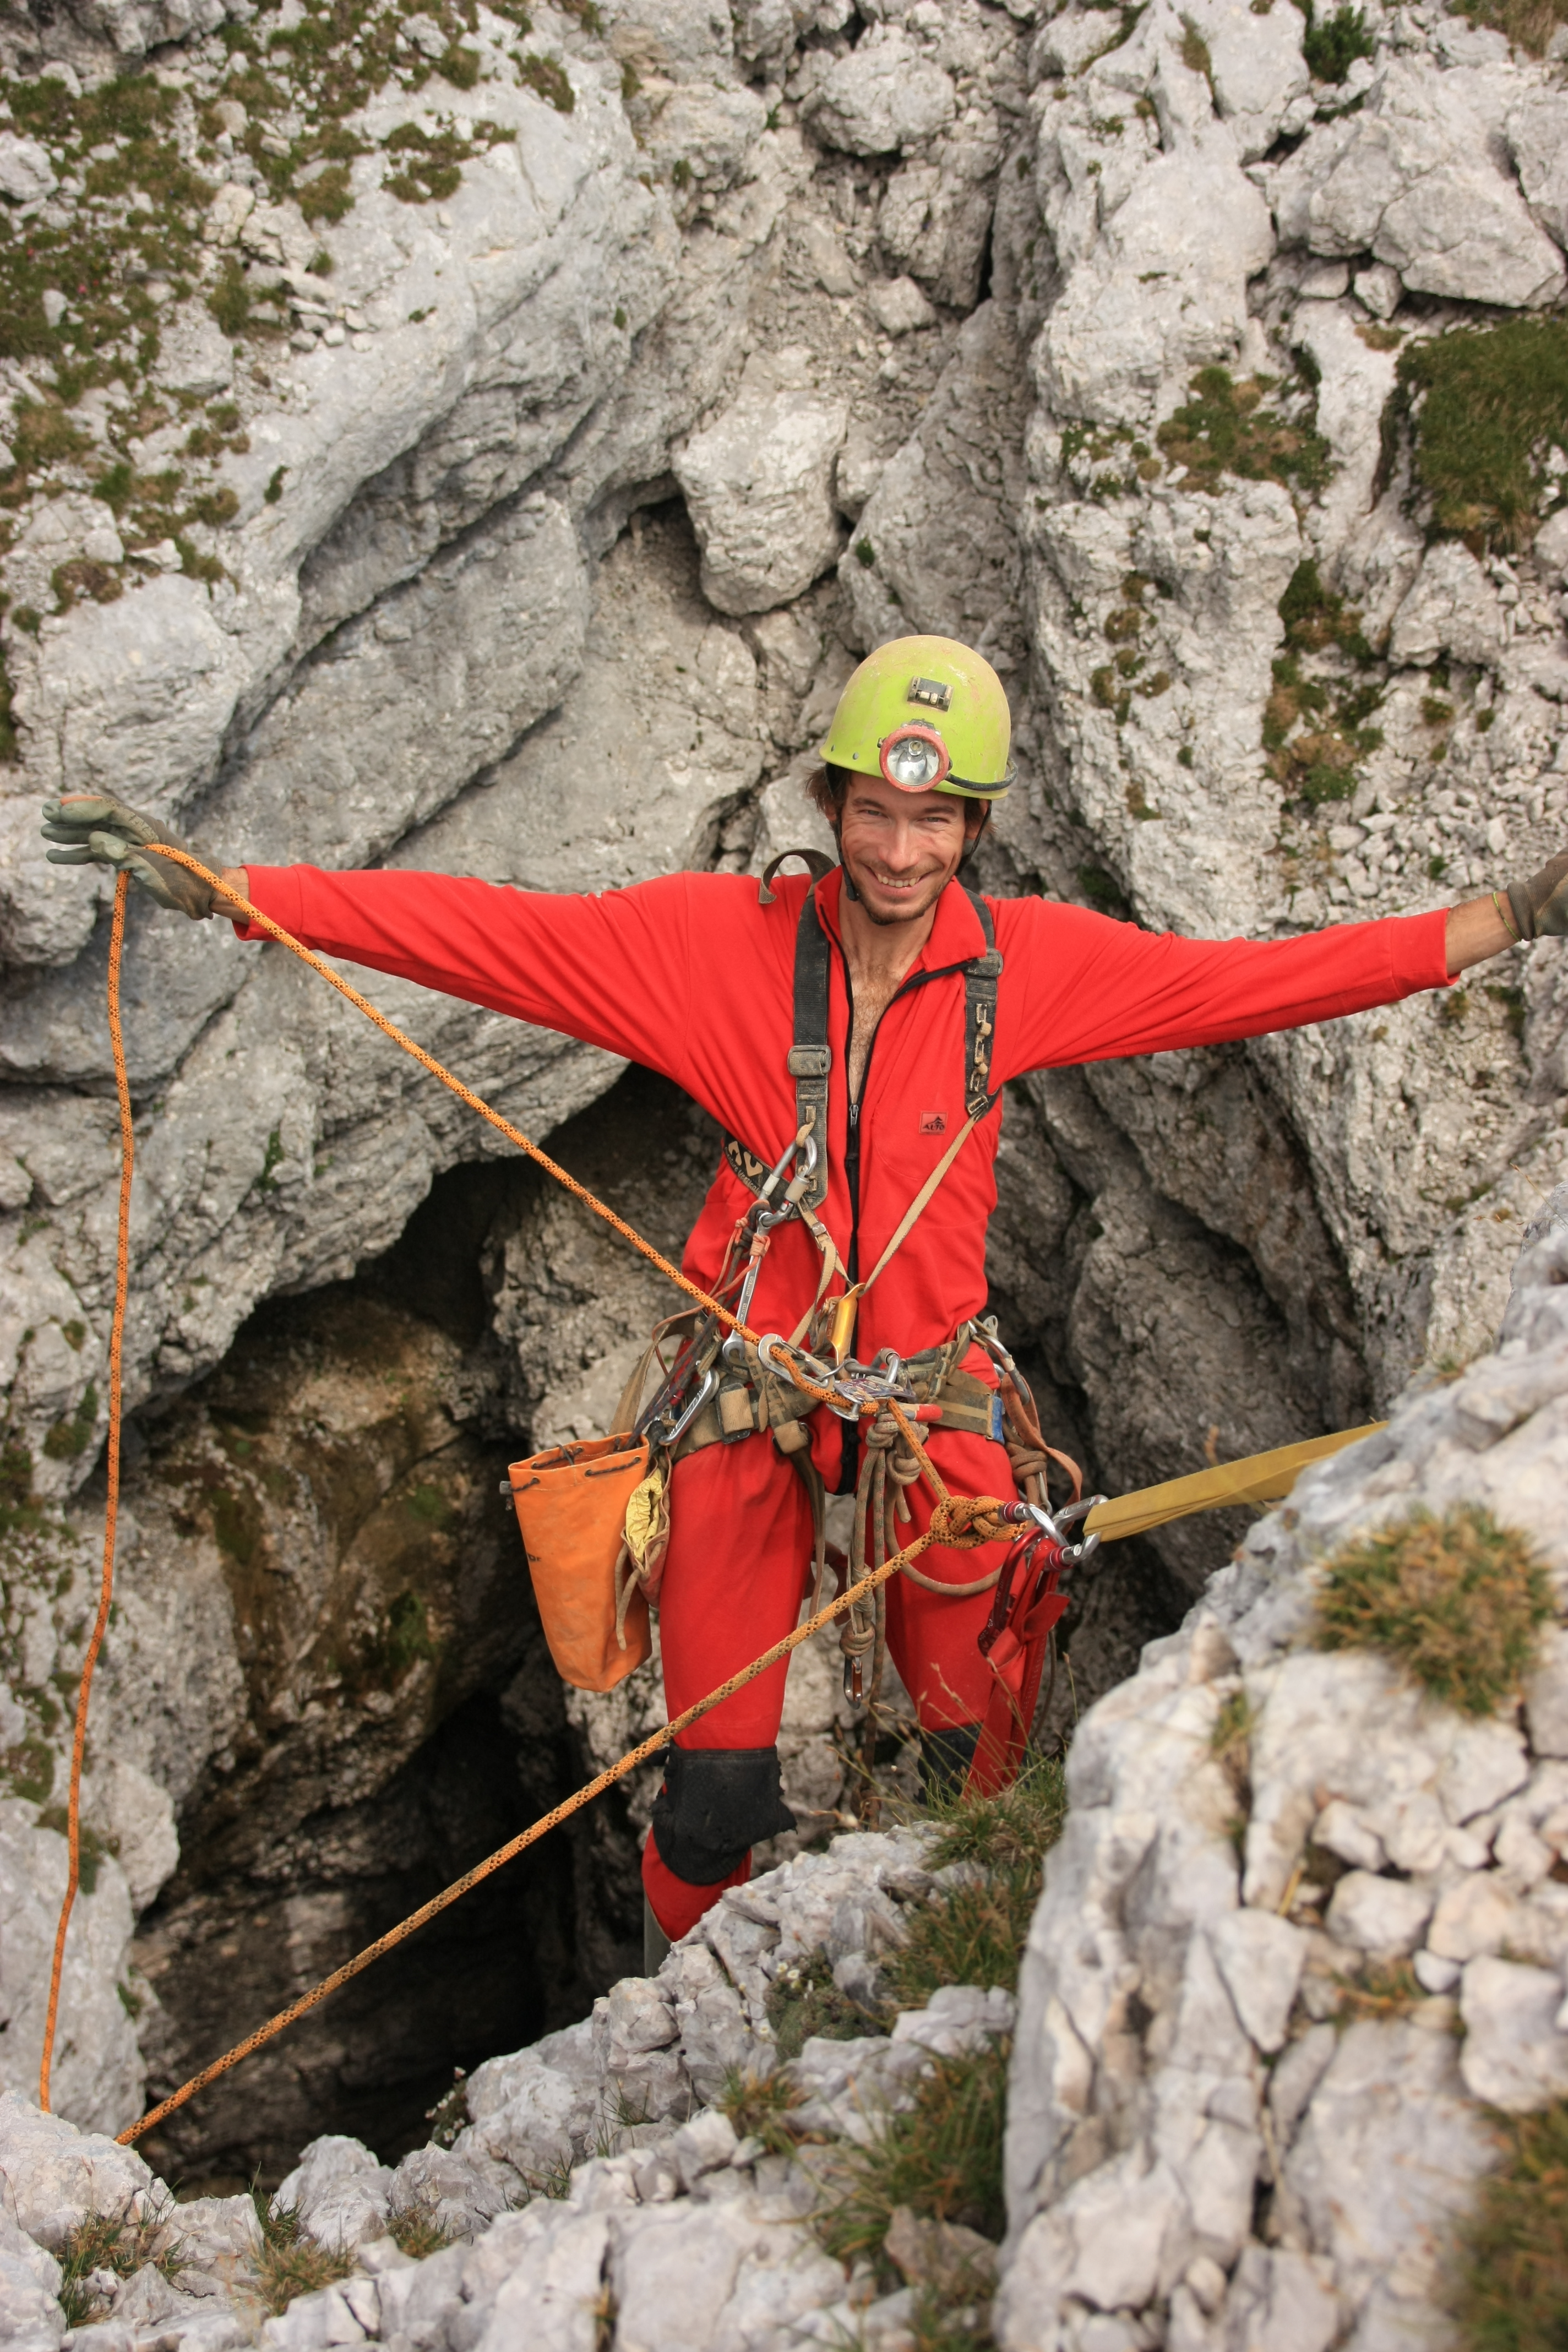
\includegraphics[width=\linewidth]{appendices/personal_equip_2007/2012-07-30-0327-GergelyAmbrus-IMG_2103--orig.jpg}} 
 \caption{Gergely in his caving gear (minus oversuit). \pic{Gergely Ambrus}}
 \label{caving equipment}
\end{marginfigure}

\textbf{To Buy for yourselves}:
\begin{itemize}
    \item Thermals – I will probably not take mine off between arriving up top and going down again \textbf{– 1}
    \item Fleecy hats, gloves and a balaclava, it can get very cold while you wait for someone else to put in a bolt. \textbf{- 1}
\end{itemize}

\textbf{SRT equipment}
\begin{itemize}
    \item Harness
    \item Cowstails \& krabs
    \item Footloop \& screwgate krab \& maillon \& safety cord
    \item Hand jammer
    \item Chest jammer \& carbine hook
    \item Chest harness
    \item Descender \& krab
    \item Breaking krab
    \item Prussik loops or spare jammer (do you know how to use them?) – Remind me to show you about knot passes and using prussic loops.
\end{itemize}
					
\textbf{Lighting – You have to buy this!}
\begin{itemize}
    \item Helmet
    \item Bisen (AKA Dave light, AKA Mig Light)
    \item Tikka (Plus)
\end{itemize}


\begin{marginfigure}
\checkoddpage \ifoddpage \forcerectofloat \else \forceversofloat \fi
\centering
 \frame{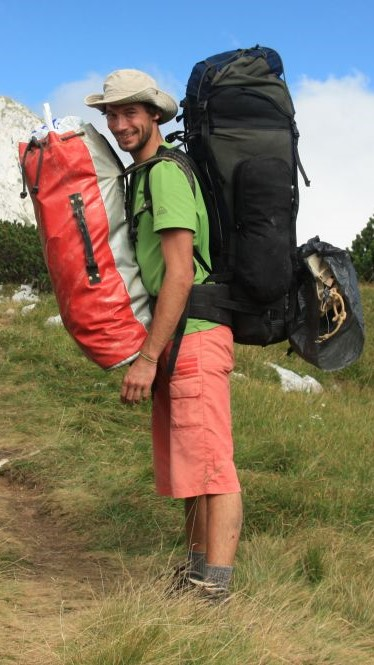
\includegraphics[width=\linewidth]{appendices/personal_equip_2007/2011-08-11-15.14.54-Gergely Ambrus-Canon450D-IMG_1392-Mountain Derig--orig.jpg}} 
 \caption{Gergely fully loaded and ready to carry all of his gear. \pic{Gergely Ambrus}}
 \label{gergely carry}
\end{marginfigure}
 
\subsection{Down the Hill}
This is mainly for the benefit of the inhabitants of Tolmin rather than us. Also, there is a nice river to swim in/sunbathe by.
\begin{itemize}
    \item Clean trousers
    \item Clean t-shirt
    \item Trainers or sandals (you can wear your boots)
    \item Socks
    \item Swimming costume
\end{itemize}

\textbf{Wash-kit (bottom)}
\begin{itemize}
    \item Shaving kit
    \item Soap
    \item Face cloth
    \item Shampoo
    \item Towel
\end{itemize}

\textbf{Miscellaneous}
\begin{itemize}
    \item Money - Solvenia has now joined the Euro
    \item Sleeping bag (or liner) for Tetley’s. You can just carry one down from the top. It's hot at night in Tolmin.
\end{itemize}

%Up top vocab: 
%Cow - Dried milk powder
%Vitaminski -  Powdered vitamin sugary fizzy drink
%TVP - Rank Soya meat substitute
%Double Rumski  - Alcohol with rum flavouring (75\% by volume)
%Vodski - Vodka
%Slop - (Cooked) Food
%Shed - Dangerous wild beast found on Slovenian mountains, occasionally found looting nearby villages
%Old Lag - Experienced member of ICCC aged 25+ 
%Schonky - Blanket adjective used to describe anything dodgy, dangerous, loose or frightening, especially in caves
%Twatty - Adjective used to describe sections of cave which are tight, annoying, unnecessarily awkward or unimpressive
%Faff - To laze, to waste time or take part in pointless labour
%Eyy -Oh All purpose non-descript salutation
%Blighty - Britain
%Comf - Noun used to describe comfortable materials to sit or lie on, in particular, it describes chopped up bits of carrymat to sit on in the bivvy
%Semtex - The cheapest cheese money can buy; on which the expedition lives
%The Orb - The Sun
%Clag - What clouds look like from the inside when enveloping the mountain
%Blue cloud - Patch of blue sky on a day of unrelenting clag

\name{Clewin Griffith}